\documentclass{article}

\usepackage[a4paper,left=18mm,right=18mm,top=20mm,bottom=18mm]{geometry}
\usepackage[italian]{babel}

\usepackage{titling}
\usepackage{graphicx}
\usepackage{subcaption}
\usepackage{float}

\title{Report analisi dell'aria}
\author{David Guzman Piedrahita e Marco Vinciguerra}
\date{\today}

\makeatletter         
\def\@maketitle{
\noindent\begin{minipage}{\textwidth}
\begin{minipage}[c]{0.8\textwidth}  
\begin{center}
{\Huge \bfseries \sffamily \@title }\\[4ex] 
{\Large  \@author}\\[4ex] 
\@date\\[0ex]
\end{center}
\end{minipage}\hfill
\begin{minipage}[c]{0.2\textwidth}
\raggedleft

\includegraphics[width = 20mm]{Picture/logo.png}\\[0.1ex]

\includegraphics[width = 25mm]{Picture/UniBg-logo.jpg}
\end{minipage}
\end{minipage}  
}
\makeatother
    

\begin{document}

\maketitle

\par\noindent\rule{\textwidth}{0.4pt}
\textbf{Abstract:} Gestione dei grafici delle centraline prese in considerazione
\par\noindent\rule{\textwidth}{0.4pt}
\section{Mappe}
\begin{figure}[H]
  \centering
  
\includegraphics[scale = 0.7]{Picture/AQStationsOfInterest.jpeg}
  \caption{ciao}
\end{figure}
\begin{figure}[H]
  \centering
  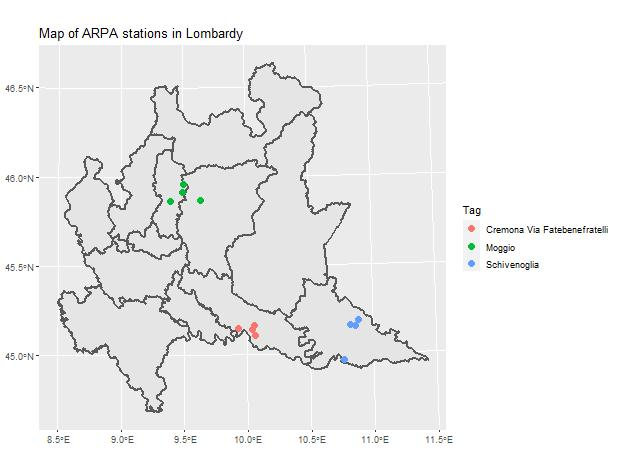
\includegraphics[scale = 0.4]{Picture/WStationsOfInterestConstrained.jpeg}
  \caption{Schivenoglia 2018-2020}
\end{figure}
\begin{figure}[H]
  \centering
  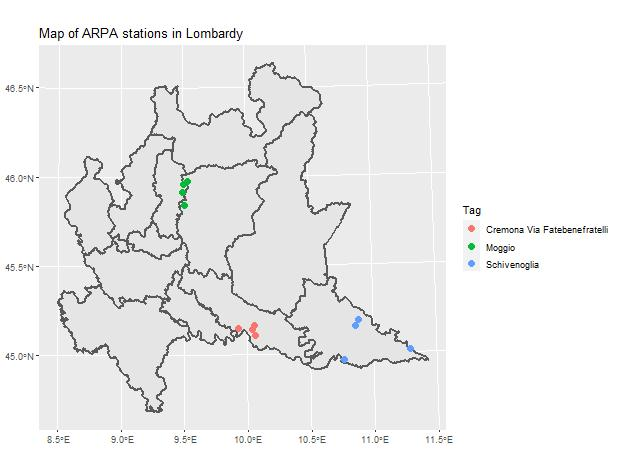
\includegraphics[scale = 0.4]{Picture/WStationsOfInterest.jpeg}
  \caption{ciao}
\end{figure}

\section{703: Schivenoglia (R)}
\subsection{Pollutants}
\begin{figure}[H]
  \centering
  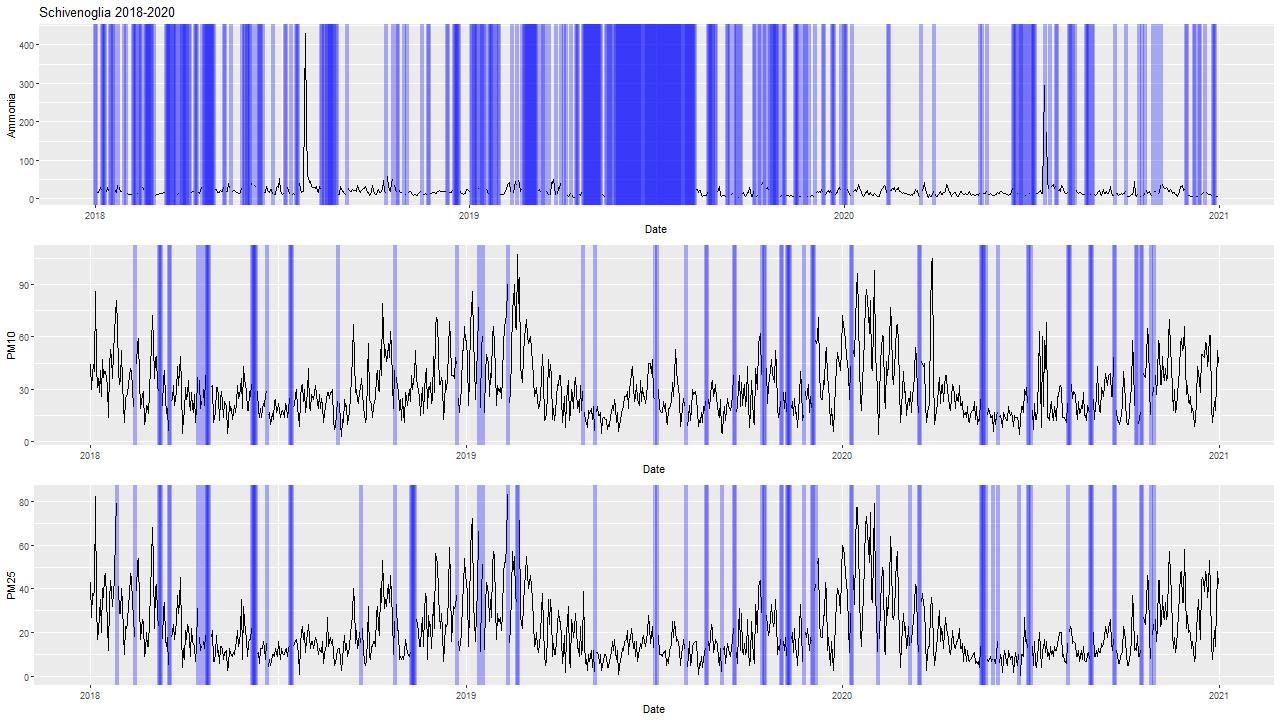
\includegraphics[scale = 0.4]{Picture/Schivenoglia 2018-2020.jpeg}
  \caption{Schivenoglia 2018-2020}
  \centering
\end{figure}
\subsection{Weather}
\subsubsection{K=1}
\begin{figure}[H]
  \centering 
  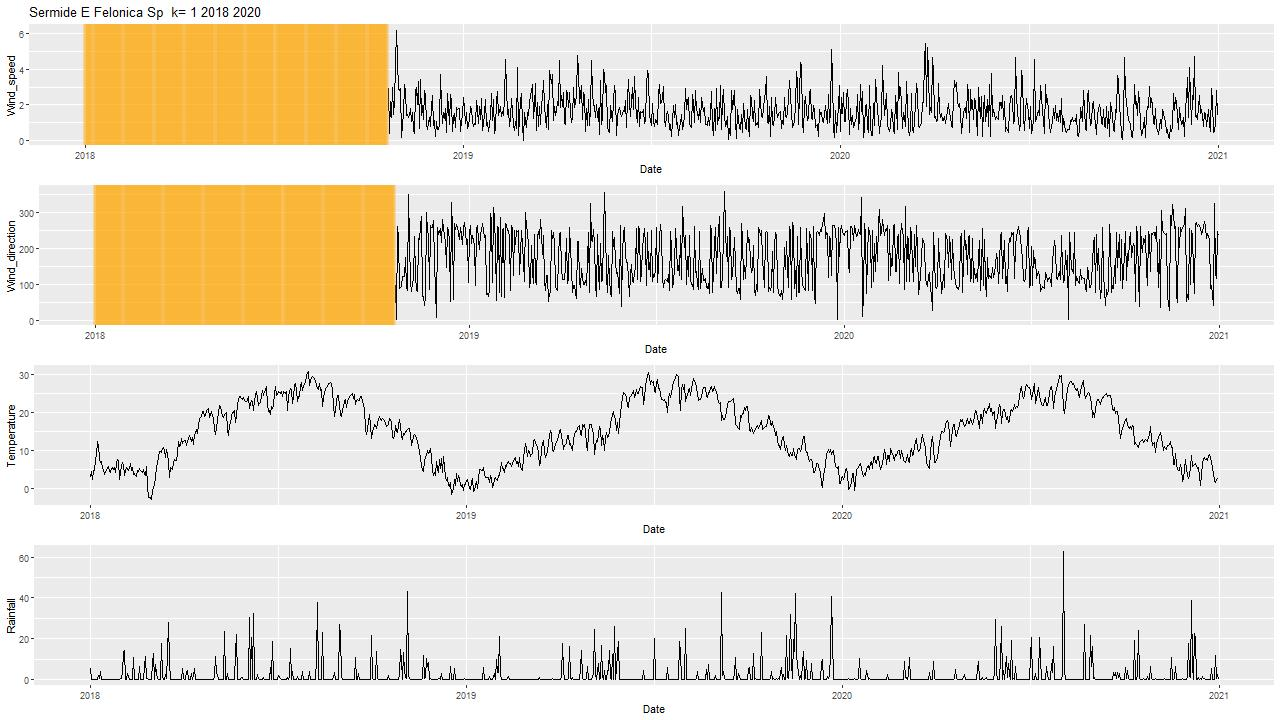
\includegraphics[scale = 0.3]{Picture/1/Sermide E Felonica .jpeg}
  \caption{Sermide E Felonica Sp  k = 1}
  \centering
\end{figure}
\subsubsection{K=2}
\begin{figure}[H]
  \centering 
  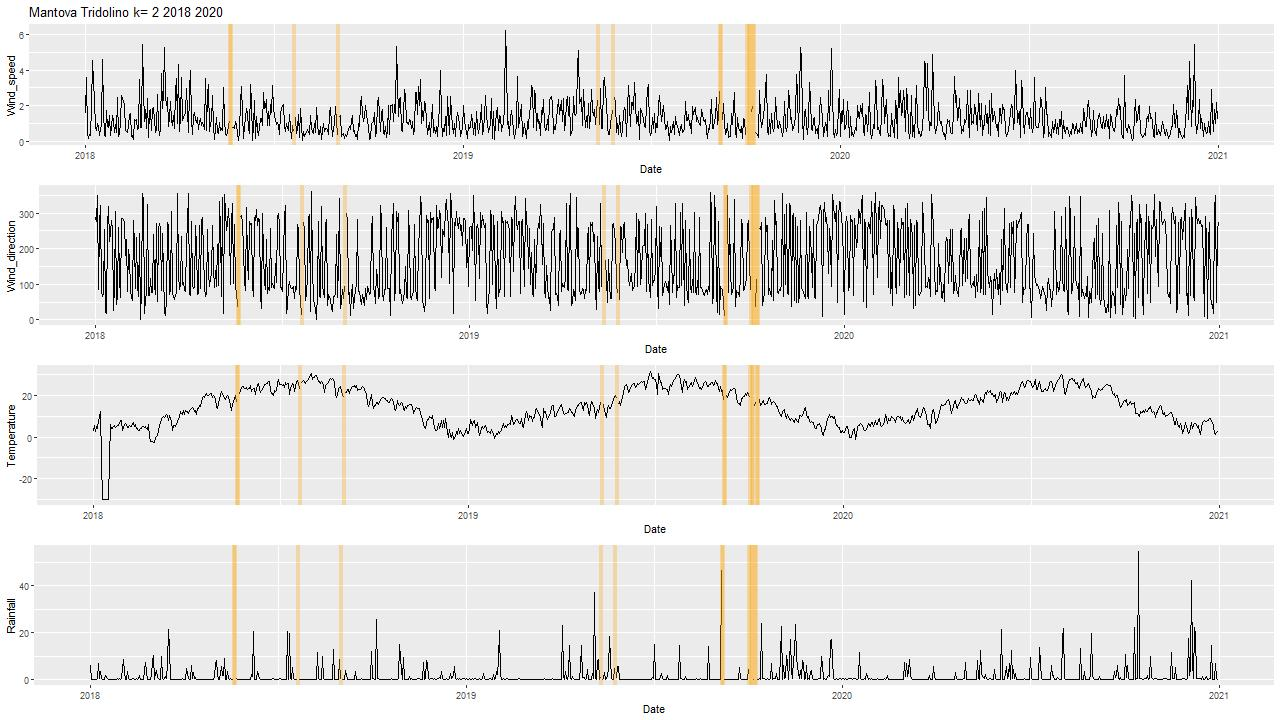
\includegraphics[scale = 0.3]{Picture/2/Mantova Tridolino k= 2 2018 2020 .jpeg}
  \caption{Mantova Tridolino k = 2}
  \centering
\end{figure}
\subsubsection{K=3}
\begin{figure}[H]
  \centering 
  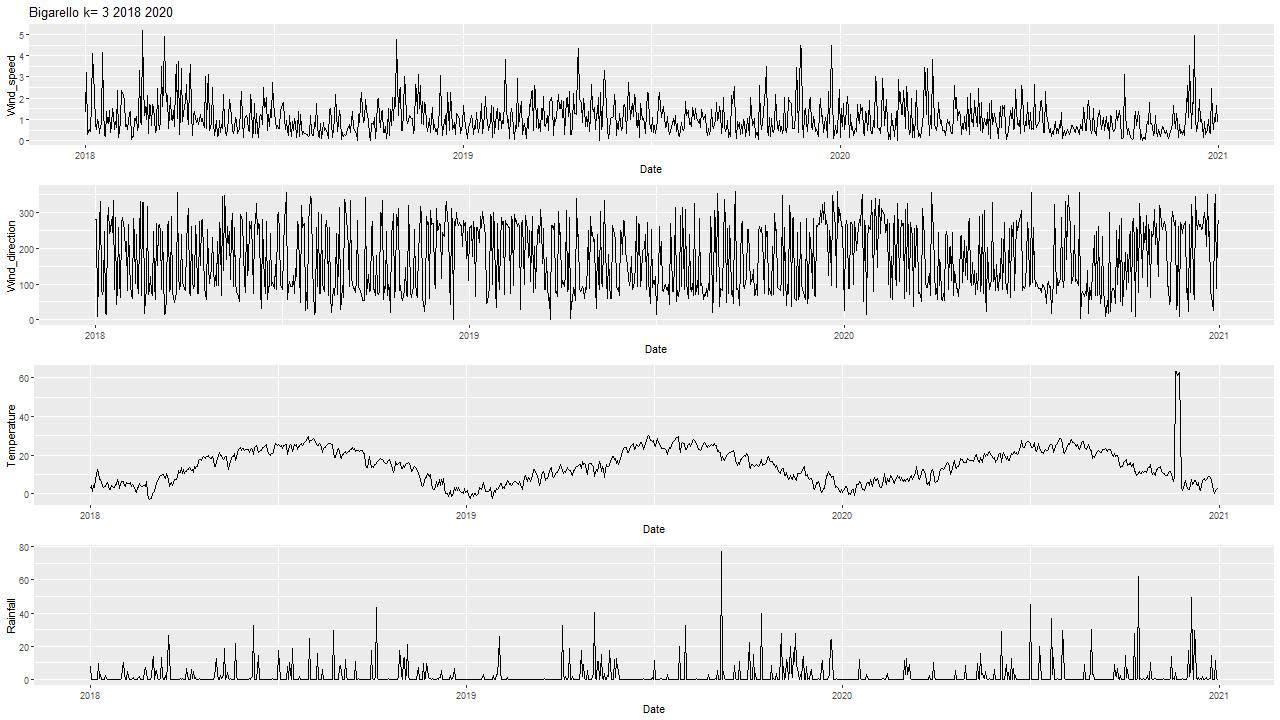
\includegraphics[scale = 0.3]{Picture/3/Bigarello k= 3 2018 2020 .jpeg}
  \caption{Bigarello k = 3}
  \centering
\end{figure}

\section{681: Moggio (R)}
\subsection{Pollutants}
\begin{figure}[H]
  \centering
  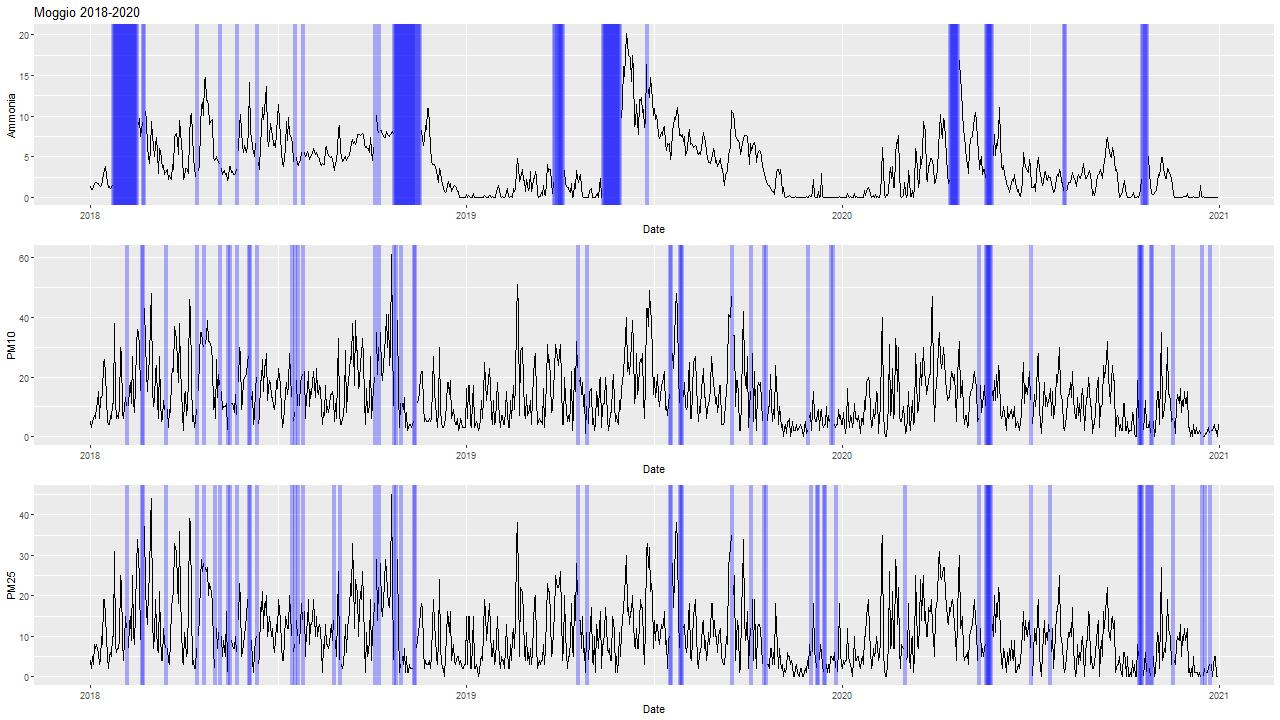
\includegraphics[scale = 0.4]{Picture/Moggio 2018-2020.jpeg}
  \caption{Moggio 2018-2020}
  \centering
\end{figure}
\subsection{Weather}
\subsubsection{K=1}
\begin{figure}[H]
  \centering 
  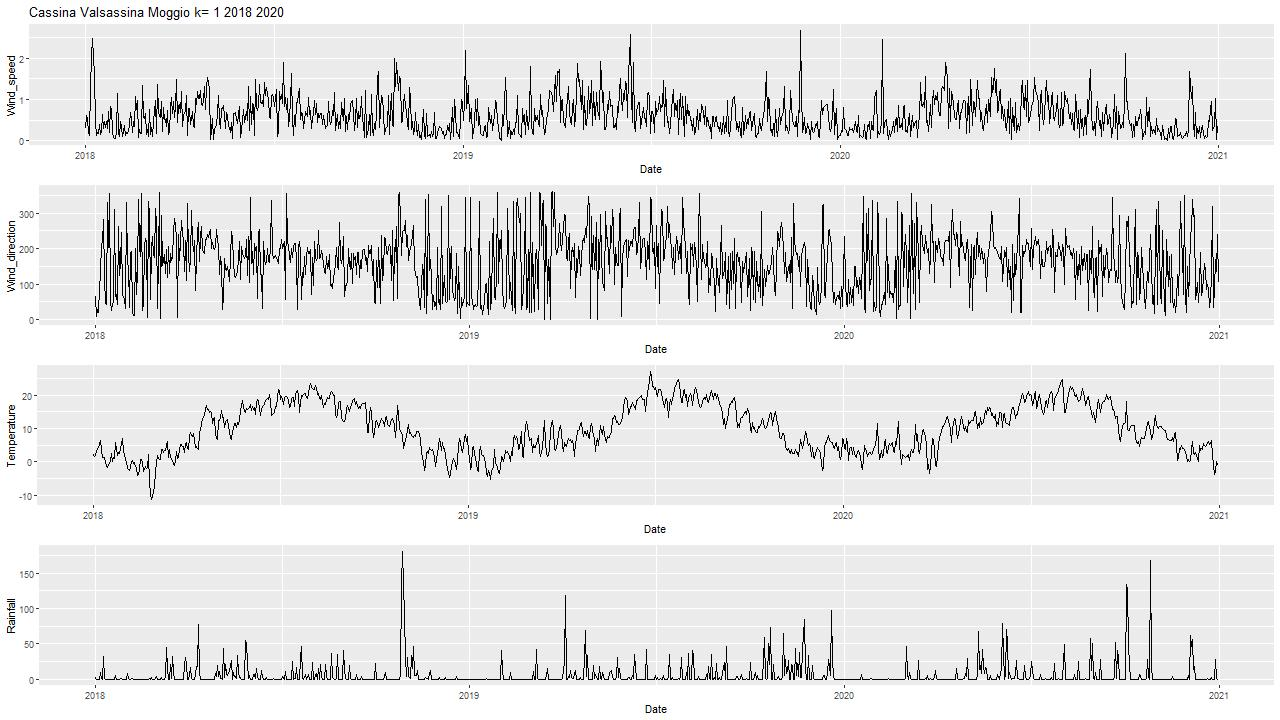
\includegraphics[scale = 0.3]{Picture/1/Cassina Valsassina Moggio k= 1 2018 2020 .jpeg}
  \caption{Cassina Valsassina Moggio k = 1 }
  \centering
\end{figure}
\subsubsection{K=2}
\begin{figure}[H]
  \centering 
  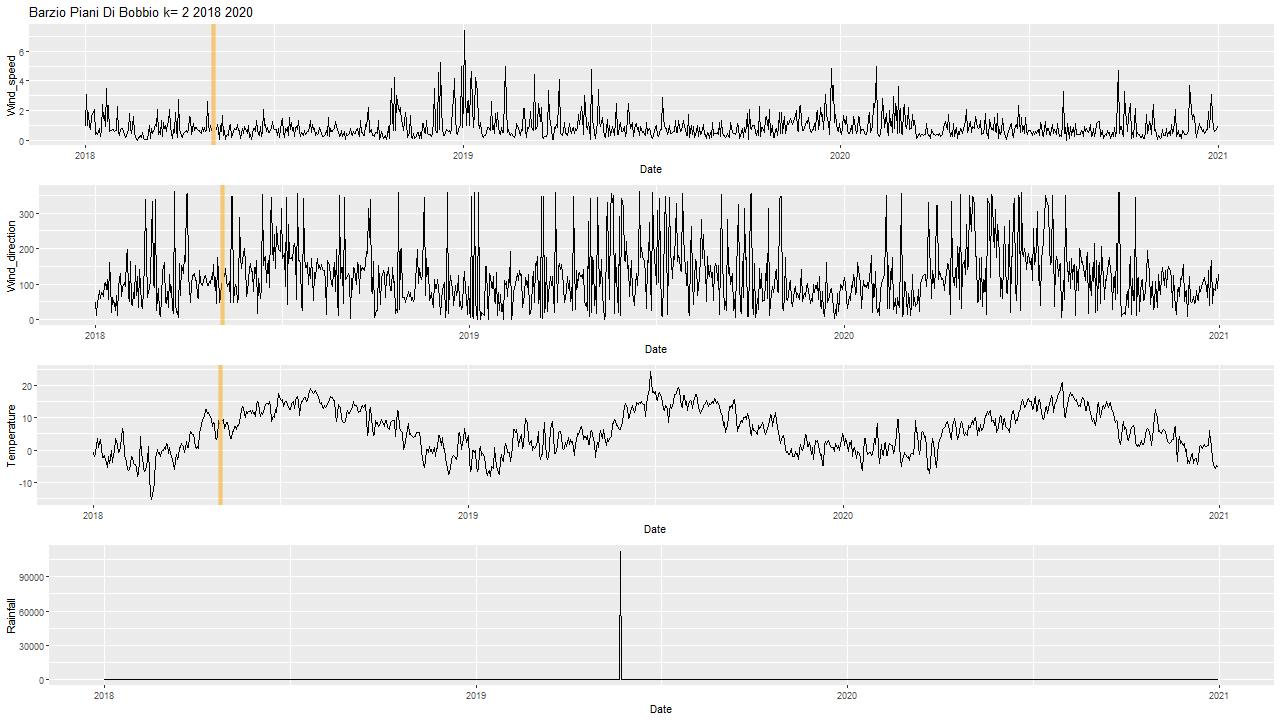
\includegraphics[scale = 0.3]{Picture/2/Barzio Piani Di Bobbio k= 2 2018 2020 .jpeg}
  \caption{Barzio Piani Di Bobbio k = 2}
  \centering
\end{figure}

\section{627: Cremona P.zza Cadorna (U)}
\subsection{Pollutants}
\begin{figure}[H]
  \centering
  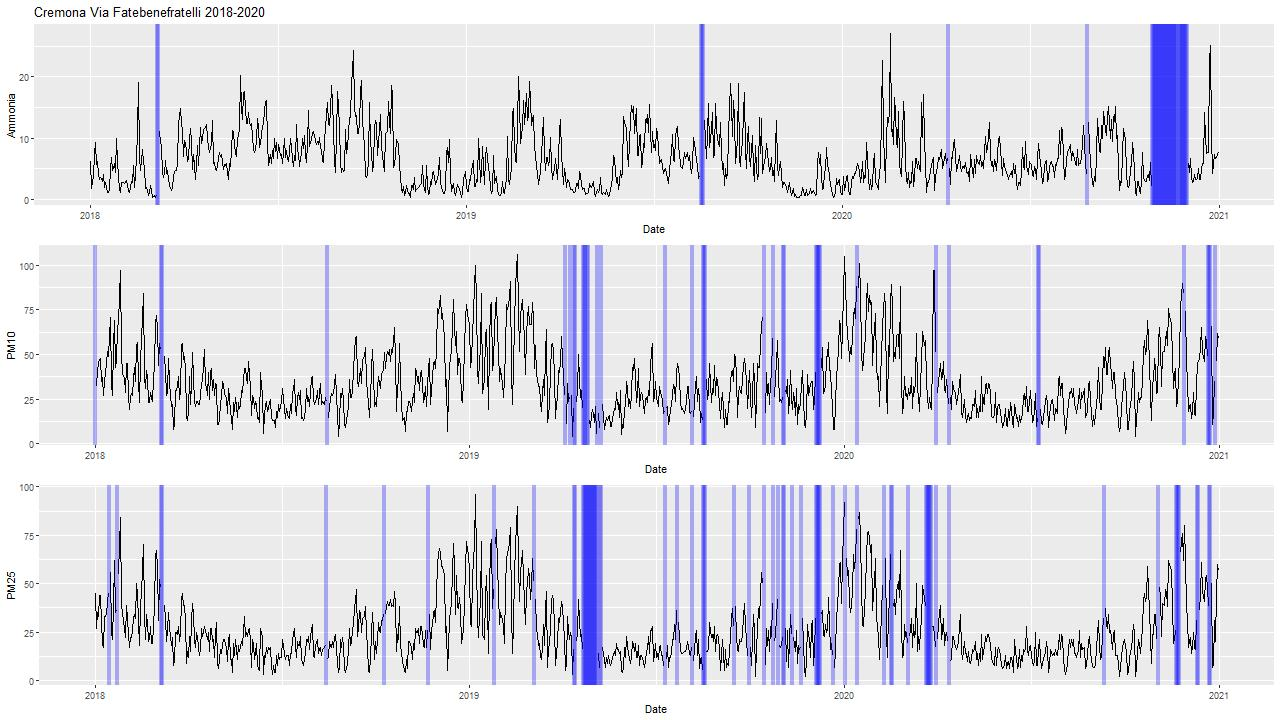
\includegraphics[scale = 0.4]{Picture/Cremona Via Fatebenefratelli 2018-2020.jpeg}
  \caption{Cremona P.zza Cadorna (U) 2018-2020}
  \centering
\end{figure}
\subsection{Weather}
\subsubsection{K=1}
\begin{figure}[H]
  \centering 
  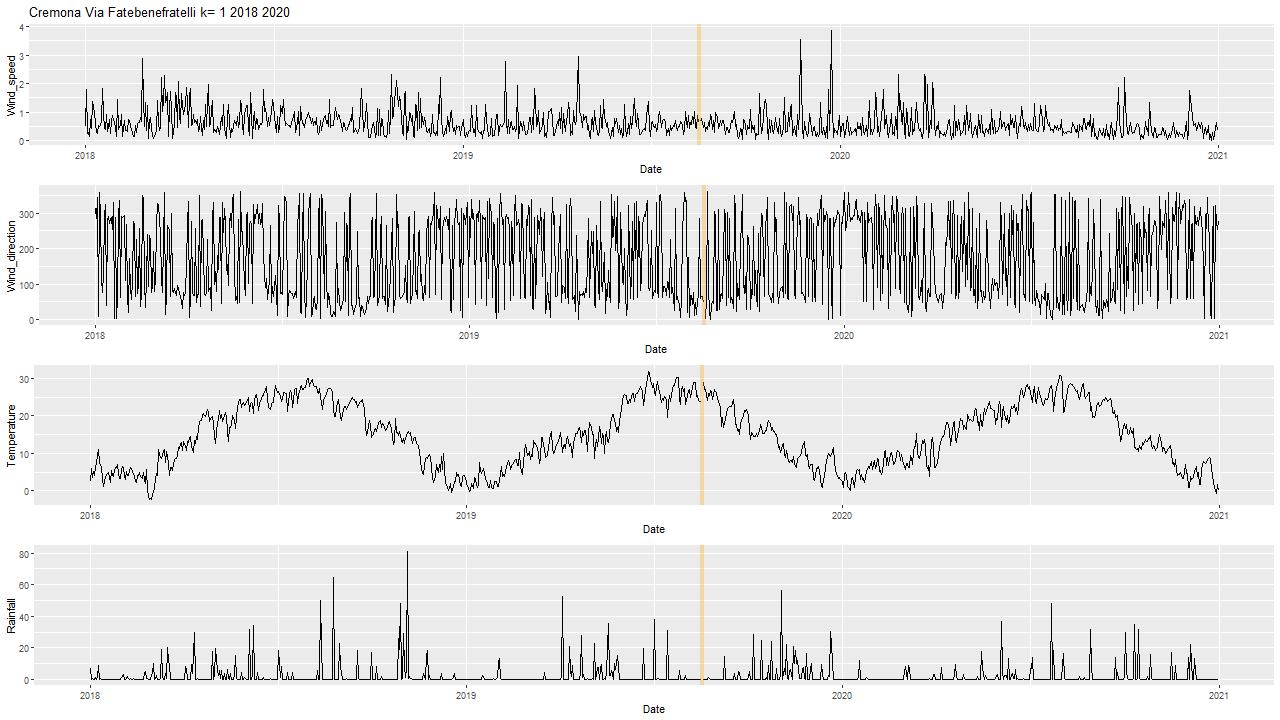
\includegraphics[scale = 0.3]{Picture/1/Cremona Via Fatebenefratelli k= 1 2018 2020 .jpeg}
  \caption{Cremona Via Fatebenefratelli k = 1}
  \centering
\end{figure}
\subsubsection{K=2}
\begin{figure}[H]
  \centering 
  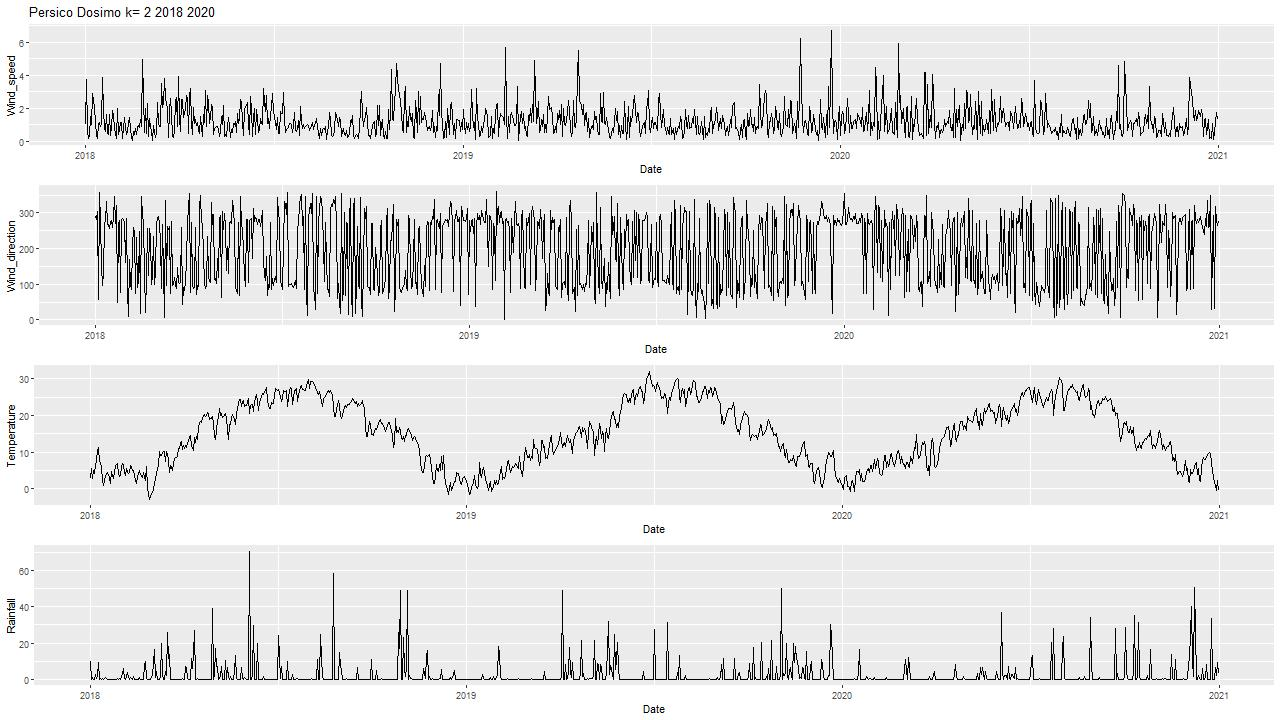
\includegraphics[scale = 0.3]{Picture/2/Persico Dosimo k= 2 2018 2020 .jpeg}
  \caption{Persico Dosimo k = 2}
  \centering
\end{figure}
\subsubsection{K=3}
\begin{figure}[H]
  \centering 
  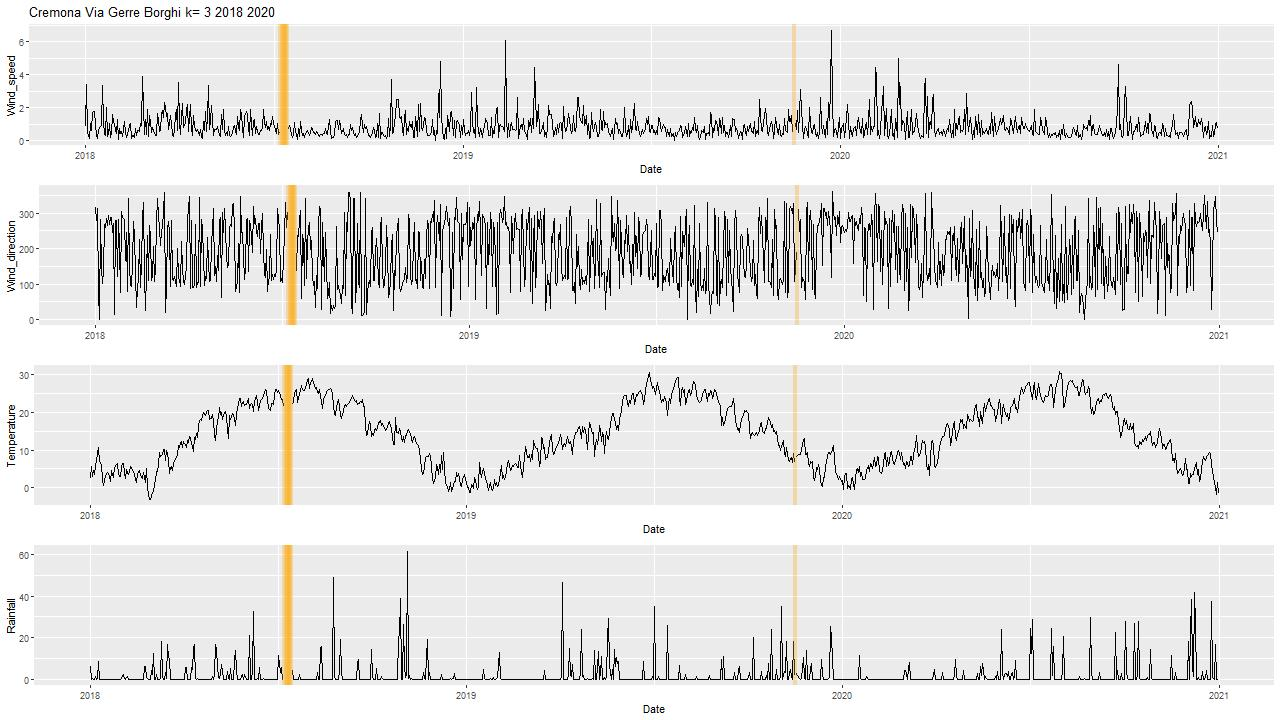
\includegraphics[scale = 0.3]{Picture/3/Cremona Via Gerre Borghi k= 3 2018 2020 .jpeg}
  \caption{Cremona Via Gerre Borghi k = 3}
  \centering
\end{figure}
\end{document}
